\documentclass[]{article}
\usepackage[T1]{fontenc}
\usepackage[latin1]{inputenc}
\usepackage[german]{babel}
\usepackage{amsmath,amsthm,amssymb,amscd,color,graphicx}
  
\theoremstyle{remark}
\newtheorem{satz}{Satz}
\newtheorem{aufg}{Aufgabe}
\newtheorem{definition}{Definition}

%opening
\title{S�tze mit Fibonaccizahlen, dem goldenen Schnitt und der Zahl 5}
\author{}

\begin{document}

\maketitle

\begin{abstract}
Eine Sammlung h�bscher und teilweise �berraschender Ergebnisse, worin Fibonaccizahlen, der goldene Schnitt oder die Zahl 5 eine besondere Rolle spielen. Keine Beweise.
\end{abstract}

\section{Fibonaccizahlen}
\begin{definition}
Die Folge $(f_n)_{n\geq 0}$ der Fibonaccizahlen ist rekursiv gegeben durch:
\begin{equation*}
f_0 = 0,\quad f_1 = 1,\quad f_{n+2} = f_{n+1} + f_{n} 
\end{equation*}
Die Folge beginnt mit
\[
0, 1, 1, 2, 3, 5, 8, 13, 21, 34, 55, 89, 144, 233, 377, 610, 987, 1597, 2584, 4181,6765, \ldots \]
\end{definition}

\begin{satz}
Die gew�hnliche und die exponentiell erzeugende Funktion der Fibonaccizahlen $G_f$ resp. $E_f$ sind:
\begin{align*}
G_f(x) :=& \sum_{n\geq 0} f_{n+1}x^n = \frac{1}{1-x-x^2}, \\
E_f(x) :=& \sum_{n\geq 0} \tfrac{1}{n!}f_n x^n = \tfrac{1}{\sqrt{5}}\exp\left(\tfrac{1+\sqrt{5}}{2}\, x\right) -
\tfrac{1}{\sqrt{5}}\exp\left(\tfrac{1-\sqrt{5}}{2}\, x\right)
\end{align*}
\end{satz}
\begin{satz} Erzeugende Funktionen von Potenzen der Fibonaccizahlen:
\begin{align*}
\sum_{n\geq 0} f_{n+1}^2x^n &= \frac{2}{5}\cdot\frac{1}{1+x}\ +\ \frac{1}{5}\cdot\frac{3-2x}{1-3x+x^2}\\
\sum_{n\geq 0} f_{n+1}^3x^n &= \frac{3}{5}\cdot\frac{1}{1+x-x^2}\ +\ \frac{2}{5}\cdot\frac{1}{1-4x-x^2} \\
\sum_{n\geq 0} f_{n+1}^4x^n &= \frac{6}{25}\cdot\frac{1}{1-x}\ +\ \frac{4}{25}\cdot\frac{3+2x}{1+3x+x^2}\ +\ \frac{1}{25}\cdot\frac{7-2x}{1-7x+x^2}\\
\sum_{n\geq 0} f_{n+1}^5x^n &= \frac{2}{5}\cdot\frac{1}{1-x-x^2}\ +\ \frac{2}{5}\cdot\frac{1}{1+4x-x^2}\ +\ \frac{1}{5}\cdot\frac{1}{1-11x-x^2}
\end{align*}
Die einzelnen Summanden haben alle eine besondere Bedeutung. Welche? Wie lautet die erzeugende Funktion einer beliebigen Potenz von Fibonaccizahlen?
\end{satz}
\begin{satz}(Wallsche Vermutung)
\[f_5 = 5 \]
Allgemeiner gibt es f�r jede positive Zahl $k$ eine positive Zahl $r$, so da� gilt:
\[ f_{r\mathbb{N}} \subset k\mathbb{N}   \] 
Bezeichnet man die kleinste solche Zahl mit $r(k)$, so gilt f�r Primzahlen $p$ vermutlich 
\[ r(p^l) = p^{l-1} r(p) \]
Insbesondere ist $f_{5^l} $ stets durch $5^l$ teilbar.
\end{satz}
\begin{satz}
Sei $B_n$ eine $n\times n$-Matrix der Form
\[
\begin{pmatrix}
1 & 1 & & &  &  \\
1 & \ddots & \ddots   & &\multicolumn{2}{c}{\text{\huge 0}}  \\
&\ddots &\ddots &\ddots  & &  \\
& &\ddots &\ddots &\ddots   &  \\
& & & \ddots &\ddots  &   1 \\
 \multicolumn{2}{c}{\text{\huge 0}}  & & &  1&  1\\
\end{pmatrix}
\] 
Dann ist die Permanente von $B_n$ gleich $ f_{n+1} $.
\end{satz}
\begin{satz} (Danke an Andrei Okunkow.)
Sei $E$ ein Vektorb�ndel auf $\mathbb{CP}^2$, das in eine exakte Sequenz
\[
0 \longrightarrow \mathcal{O}^s \stackrel{M}{\longrightarrow} \mathcal{O}(1)^{r+s} \longrightarrow E \longrightarrow 0
\]
pa�t. ($M$ ist eine allgemeine Matrix aus Linearformen.) Dann ist $E$ semistabil (d.h. $\tfrac{\chi(U(n))}{\dim U}\leq\tfrac{\chi(E(n))}{\dim E}$ f�r Unterb�ndel $U$ von $E$ und gro�e $n$) genau dann, wenn 
\[
\frac{s}{r}\ \in\  \left\{\frac{0}{1},\frac{1}{2},\frac{3}{5},\frac{8}{13},\frac{21}{34},\ldots \right\} \cup \left\{ \alpha\ |\ \alpha > \frac{1}{\Phi} \right\}
\]
\end{satz}

\section{Goldener Schnitt}
\begin{definition}
Der goldene Schnitt $\Phi$ ist definiert als $\Phi := \tfrac{1+\sqrt{5}}{2}$. 
\end{definition}
\begin{satz}
Der goldene Schnitt erf�llt die Gleichungen
\[
\Phi = 1 + \frac{1}{\Phi}, \qquad \Phi^{n+1} = f_{n+1}\Phi + f_n.
\]
\end{satz}

\begin{satz}
Sei $f : \mathbb{R}^{\geq 0} \longrightarrow\mathbb{R}^{\geq 0} $ diejenige differenzierbare und bijektive Funktion, deren erste Ableitung gleich ihrer Umkehrfunktion ist. Dann ist $f$ gegeben durch:
\[
f(x) = \left(\tfrac{1}{\Phi}\right)^{\tfrac{1}{\Phi}} x^\Phi.
\]
\end{satz}
\begin{satz}
Sei einem regelm��igen Ikosaeder ein regelm��iges Dodekaeder einbeschrieben (Seitenfl�chenmittelpunkte auf Ecken). Dann ist das Verh�ltnis der Kantenl�ngen beider Objekte gleich $3:\Phi$.
\end{satz}
\begin{satz}
Die dreidimensionale Rotation um $72� = \frac{2\pi}{5}$ hat Spur $\Phi$. Die zweidimensionale Rotation um $72�$ hat Spur $\frac{1}{\Phi}$.
\end{satz}
\section{Die Zahl 5}
\begin{definition}
Die Zahl $5$ ist die Anzahl nicht�hnlicher platonischer K�rper.
\end{definition}
\begin{satz} (Pentagonalzahlensatz.) Die Pentagonalzahlen sind definiert durch $p_n := \tfrac{3n^2-n}{2}$ und berechnen die Anzahl der Steine, die ben�tigt werden, um $n$ ineinander liegende regelm��ige F�nfecke zu legen, welche eine Ecke gemeinsam haben.\\
Die Partitionszahlen werden bezeichnet durch $p(n)$ und z�hlen die M�glichkeiten, die Zahl $n$ als Summe positiver ganzer Zahlen zu schreiben. Dann gilt:
\begin{align*}
\frac{1}{(1-x)(1-x^2)(1-x^3)(1-x^4)\ldots} &= \sum_{n\geq 0} p(n) \,x^n\qquad \text{und} \\
(1-x)(1-x^2)(1-x^3)(1-x^4)\ldots &= \sum_{n \in \mathbb{Z}} (-1)^n x^{p_n}.
\end{align*}
\end{satz}
\begin{satz} (F�nferschritte bei Partitionszahlen.)
\[
\frac{5\left((1-x^5)(1-x^{10})(1-x^{15})\ldots \right)^5 }{\left((1-x)(1-x^2)(1-x^3)(1-x^4)\ldots\right)^6} 
= \sum_{n\geq 1} p(5n-1)\,x^n
\]
\end{satz}

\begin{satz}
(Danke an Vadim Gorin.) Sei $D$ ein Dreieck mit ganzzahligen Seitenl�ngen und einem rechten Winkel. Dann ist die kleinstm�gliche Hypothenusenl�nge gleich 5.
\end{satz}
\begin{figure}[ht]
\centering
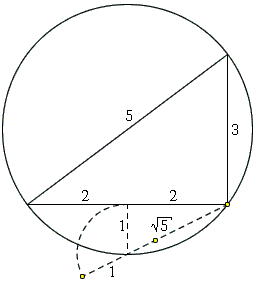
\includegraphics[scale=0.6]{3-4-5_1.png}
\end{figure}
\end{document}
